The question of how wars end has occupied strategic thinkers for centuries. Alfred Thayer Mahan's influential treatise on sea power argued that naval supremacy, expressed through decisive fleet engagements, determines the outcomes of wars and shapes the fate of nations \citep{mahan1890}. In this view, the decisive battle is the mechanism through which political objectives are achieved: destroy the enemy's capacity to fight, and the war is won. The opposing view, rooted in Clausewitz's observations and refined by modern scholars of attrition warfare, holds that wars are decided not by single moments of brilliance but by the gradual exhaustion of an adversary's material and human resources \citep{clausewitz1832}. In this framework, decisive battles are rare anomalies; most wars are won by the side that can sustain losses longer.

These two hypotheses, decisive shock versus strategic exhaustion, carry profoundly different implications for military strategy, resource allocation, and foreign policy. If wars are decided by decisive battles, then investment in elite military capabilities and offensive doctrine is warranted. If wars are decided by exhaustion, then industrial capacity, logistics, and political will become the decisive factors. Yet the empirical literature has largely treated this as a binary classification problem: each war is either ``decisive'' or ``attritional,'' with limited attention to the possibility that both mechanisms operate simultaneously at different phases of conflict.

This paper's key contribution is suggesting that decisive events and attritional processes are not competing explanations but interacting mechanisms occurring at different phases of conflict. Attrition changes the state space, degrading military capacity, eroding economic resilience, and undermining political will, and decisive shocks exploit the altered state space. The historical mistake is treating the visible collapse event as the entire cause, when it often operates atop an attritional substrate that has already shifted the strategic balance (Figure~\ref{fig:conceptual}).

\begin{figure}[ht]
\centering
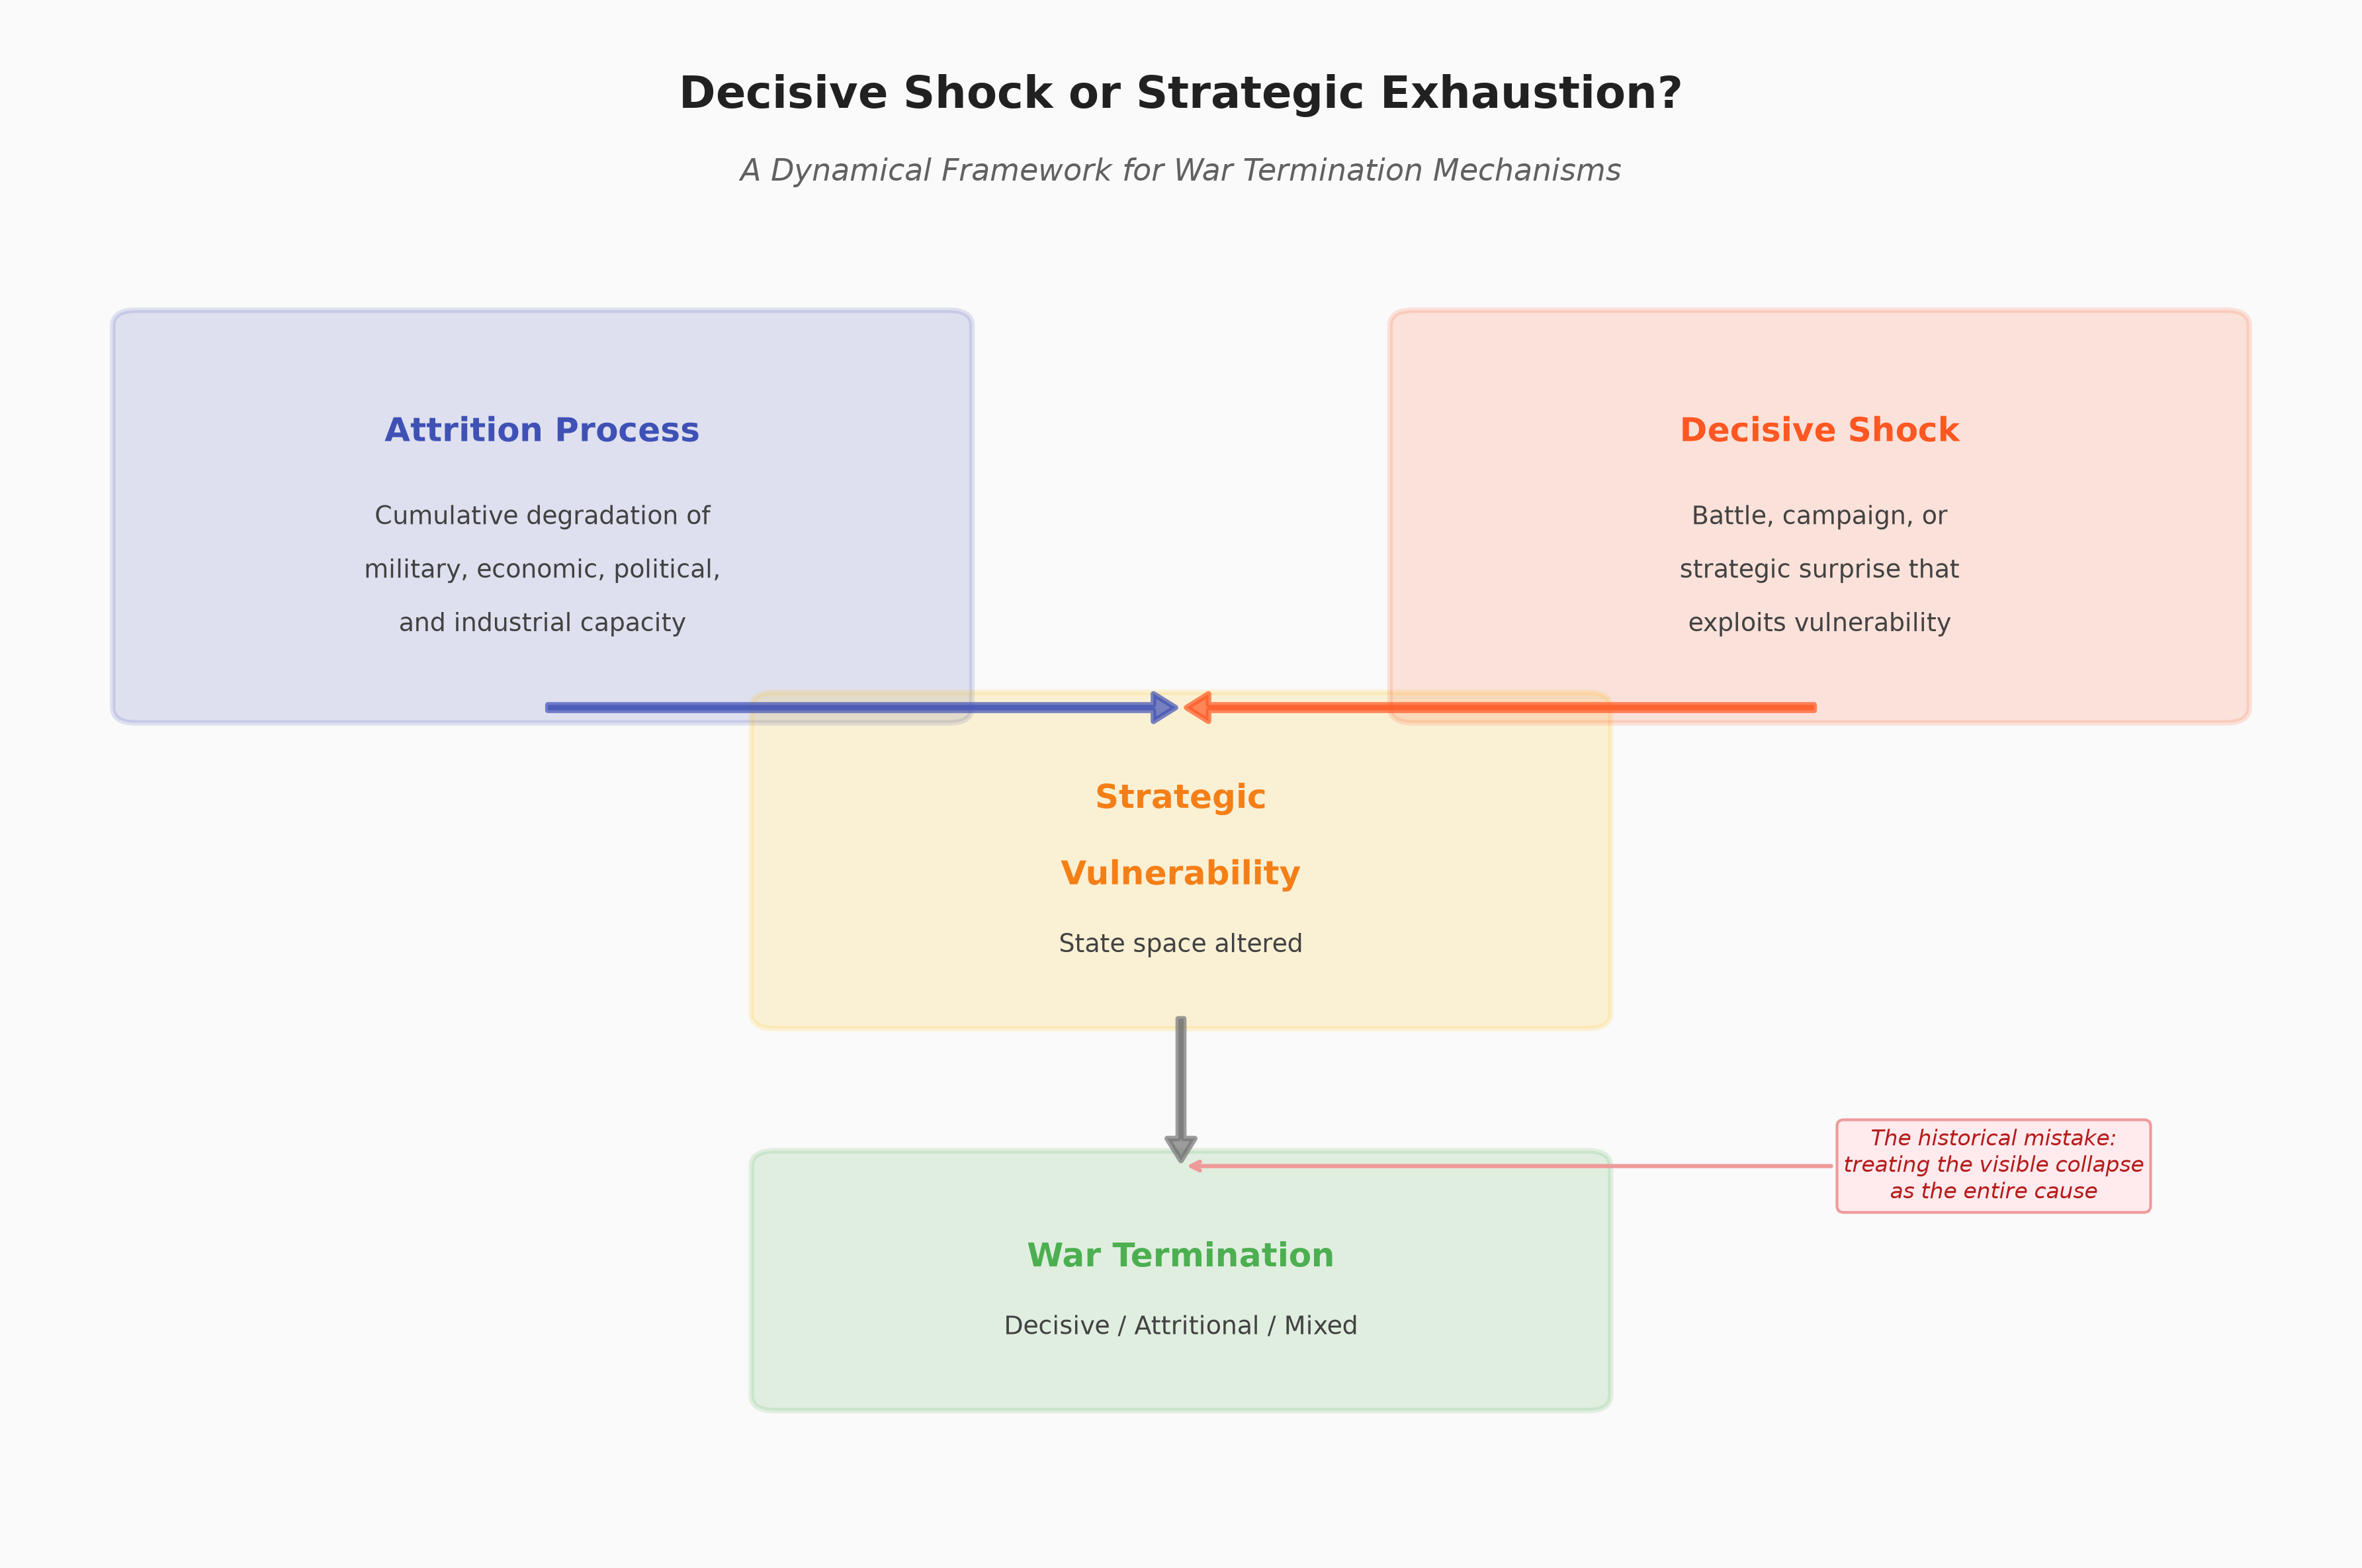
\includegraphics[width=0.8\textwidth]{figures/fig_01_conceptual_model.png}
\caption{Conceptual model of the attritional iceberg. The visible decisive shock operates atop a larger attritional substrate that has already shifted the strategic balance.}
\label{fig:conceptual}
\end{figure}

To test this framework, we develop a computational approach comprising three components: (1) the Decisive Shock Score (DSS), which quantifies the role of decisive battles or campaigns in war outcomes (noting that some DSS components require post-hoc information); (2) the Strategic Exhaustion Score (SES), which measures cumulative attritional dynamics; and (3) a dynamical simulation model that generates synthetic war trajectories under varying parameter regimes. We apply these tools to a comprehensive dataset covering 4,812 wars from antiquity to the modern era, enabling large-n quantitative analysis of war termination mechanisms.

\subsection{What the Model Generates (and What It Does Not)}

The model's classification target is deliberately narrow. It generates:

\begin{itemize}
    \item \textbf{Termination pathway class}: whether a war is more likely to terminate through decisive shock, strategic exhaustion, or a mixed process.
    \item \textbf{Dominance of mechanism}: which mechanism, shock or attrition, dominates at each phase of the conflict.
    \item \textbf{Trajectory shape}: the qualitative pattern of state variable evolution over time.
\end{itemize}

The model does \emph{not} attempt to generate:

\begin{itemize}
    \item The exact winner of a specific conflict.
    \item The date of surrender or ceasefire.
    \item Battlefield-level outcomes or tactical events.
    \item The specific battles that will occur or their timing.
\end{itemize}

This narrow classification target reflects a deliberate scientific choice. Clausewitzian strategic outcomes emerge from many interacting systems: leadership, intelligence, geography, technology, domestic politics, weather, and chance. No parsimonious model can capture all of these. Rather than claiming broad predictive power, we focus on identifying qualitative mechanism classes and the structural conditions under which each dominates.

\subsection{What This Paper Does and Does Not Claim}

\begin{table}[H]
\centering
\small
\setlength{\tabcolsep}{4pt}
\renewcommand{\arraystretch}{1.12}
\caption{Claim scope: what this paper does and does not claim. The distinction between internal model consistency and independent empirical validation is central to interpreting the results.}
\label{tab:scope}
\begin{tabularx}{\textwidth}{@{}
>{\RaggedRight\arraybackslash}p{0.20\textwidth}
>{\RaggedRight\arraybackslash}X
>{\RaggedRight\arraybackslash}X
@{}}
\toprule
\textbf{Claim type} & \textbf{Paper does claim} & \textbf{Paper does not claim} \\
\midrule
DSS/SES & Transparent scoring framework using normalized, dimensionless indices & Ground-truth taxonomy of wars \\
Simulation & Mechanism plausibility demonstration & Precise historical reconstruction \\
Case studies & Calibrated comparison with author-assigned labels & Independent historian validation \\
RF/LR & Duration prediction baseline showing nonlinear structure & Test of DSS/SES superiority \\
Attritional iceberg & Pattern in 91 wars with complete battle-level data & Universal law of war \\
Mechanism classifier & Internal consistency check (6/7 agreement) & Independent predictive accuracy \\
\bottomrule
\end{tabularx}
\end{table}

We find several key results. First, a logistic regression model using ten material-capability features (CINC scores, military expenditure, energy consumption, military personnel, iron and steel production, and their percentage changes) achieves 55.0\% cross-validated accuracy (AUC = 0.551) in predicting war duration category, only 2.7 percentage points above the null baseline of 52.3\%, while a random forest achieves 72.7\% accuracy, demonstrating that nonlinear interactions among material-capability features contain substantial predictive information that linear models cannot capture. Battle deaths are excluded from both models as wartime outcomes, not ex-ante predictors. Second, our mechanism classifier agrees with author-assigned labels in 6 of 7 cases by separating termination events from strategic causes. Third, the simulation provides a mechanistic demonstration that DSS and SES can emerge from interacting attritional and shock processes: when calibrated to historical initial conditions, the model produces trajectory classes consistent with the mechanism-trajectory classifier in 6 of 7 cases. This demonstration is consistent with internal model consistency while also revealing the fundamental difficulty of generating specific historical outcomes with simplified models.

The remainder of this paper is organized as follows. Section~\ref{sec:background} reviews the theoretical literature on war termination. Section~\ref{sec:data} describes our multi-source dataset. Section~\ref{sec:methods} details the DSS, SES, and simulation methodology. Section~\ref{sec:results} presents our empirical findings. Section~\ref{sec:discussion} interprets the results in light of existing theory, and Section~\ref{sec:conclusion} concludes with directions for future research.
